%% A simple template for a lab or course report using the Hagenberg setup
%% based on the standard LaTeX 'report' class
%% äöüÄÖÜß  <-- no German Umlauts here? Use an UTF-8 compatible editor!

%%% Magic comments for setting the correct parameters in compatible IDEs
% !TeX encoding = utf8
% !TeX program = pdflatex 
% !TeX spellcheck = en_US
% !BIB program = biber

\documentclass[english,notitlepage,smartquotes]{hgbreport}
% Admissible options in [..]: 
%   Type of document: 'diploma', 'master' (default), 'bachelor', 'internship' 
%   Main language: 'german' (default), 'english'
%		Turn on smart quote handling: 'smartquotes'
%	  Use APA bibliography style: 'apa'
%%%----------------------------------------------------------

\RequirePackage[utf8]{inputenc}		% remove when using lualatex oder xelatex!
\renewcommand{\chapter}[1]{}	% \chapter is deactivated

\graphicspath{{images/}}   % where are the images?

\bibliography{references}   % requires file 'references.bib'
\ExecuteBibliographyOptions{backref=false}



%%-----------------------------------------------------------
\setcounter{chapter}{3}	% <----- set to assignment number!
%%-----------------------------------------------------------

\author{Alex A.\ Wiseguy}
\title{MTD362 Digital Imaging -- WS 2020/21\\
				Lab Report \arabic{chapter}}
\date{\today}


%%%----------------------------------------------------------
\begin{document}
%%%----------------------------------------------------------
\maketitle
%%%----------------------------------------------------------

\begin{abstract}\noindent
This lab unit deals with various interesting problems  \ldots 
(give a short summary of the specific topics addressed).
If you decide to write your report in German, make sure to
change the \verb!\documentclass! parameter from \texttt{english}
to \texttt{german}.
If you write in MS Word (and such), try to use a similar structure.
\end{abstract}



\section{The first assignment}

Describe the goals of the assignment briefly in your own words
(i.e., do not just copy-paste the assignment text).
In general, try to describe
\begin{itemize}
\item
	the task or problem to solve;
\item
	the details of your solution, key ideas, steps involved, math, algorithms,
	references, \ldots ;
\item
	tests used to validate your solution and/or performance.
\end{itemize}

\subsection{Structuring}	% title of a subtask

This \latex document is based on the \texttt{HagenbergThesis} 
template, whose most recent version can be found on GitHub.%
\footnote{\url{https://github.com/Digital-Media/HagenbergThesis}}

The document uses the custom class \textsf{hgbreport} which is based
on \latex's standard \texttt{report} document class. Each lab unit 
(weekly assignment) corresponds to one \texttt{chapter}.
Use \verb!\setcounter{chapter}{n}! in the document's preamble
to set the \emph{lab unit number} to \texttt{n}.
Note that the \verb!\chapter! command itself is deactivated.
Use \verb!section{..}! at the beginning of each \emph{assignment}.
For individual \emph{subtasks} use the 
\verb!\subsection{..}! command, as shown here.



\subsection{Literature}

Use \emph{references} to literature or online resources whenever you found 
something relevant.
For example, the textbook recommended for this course is \cite{Sedgewick2011}.


\subsection{Mathematical elements}

Use mathematical expressions wherever appropriate, either in-line 
(e.g., $e = m \cdot c^2$) or in the form of displayed equations, such as
%
\begin{equation}
	e = m \cdot c^2 .
\end{equation}




\subsection{Pictures, figures}

Uses figures to show your test images, results, screen shots etc.,  
noting that (with the given setup) only
graphics in PNG, JPEG and PDF format can be directly included
(see Fig.~\ref{fig:example}).
See the thesis template for more details.
All images are set up to reside in the \verb!images/! subdirectory.
However, it may be a good idea to create a specific image folder for
each assignment.

\begin{figure}[htbp]
\centering\small
\begin{tabular}{cc}
	\fbox{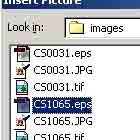
\includegraphics[width=0.45\textwidth]{screenshot-dirty}} &		% JPEG file
	\fbox{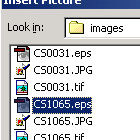
\includegraphics[width=0.45\textwidth]{screenshot-clean}} \\	% PNG file
	(a) & (b) 
\end{tabular}
\caption{Example for including images in a figure. Explain what is shown
in (a) and (b), respectively.} 
\label{fig:example}
\end{figure}



\subsection{Including code}

Include relevant code snippets as shown in this Java example:
%
\begin{JavaCode}[numbers=none]
import ij.ImagePlus;
import ij.plugin.filter.PlugInFilter;
import ij.process.ImageProcessor;

public class Filter_Demo implements PlugInFilter {
	
	public int setup(String arg, ImagePlus imp) {
		return DOES_ALL;	// works for any type of image!
	}

	public void run(ImageProcessor ip) {
		float[] H = { 		// this is a 1D array!
				1, 2, 1,
				2, 4, 2,
				1, 2, 1 
		};
		ip.convolve(H, 3, 3);		// a 3 x 3 filter kernel
	}
}
\end{JavaCode}
%
The thesis template provides suitable code environments for
various other languages.


\section{The second assignment}

And so on for all other assignments \ldots


\section*{Summary and comments}

Here you should summarize your learning experience,
personal discoveries and major difficulties (if any).
Also state the approximate amount of time you spent for
this assignment and any optional accomplishments.
This non-numbered section is produced with the
\verb!\section*{..}! command.
 



%%%----------------------------------------------------------
  
\section*{References}
\printbibliography[heading=noheader]

%%%----------------------------------------------------------

\end{document}
